
\chapter{FDTD} \label{ch:fdtd}


FDTD expresses Maxwell's equations as a set of discretized time-domain equations\cite{Yee}. These equations describe each electric field component in terms if its orthogonal, coupled magnetic fields, and each magnetic field component as a function of its coupled electric fields.


\section{Wave equation}

In a time-domain simulation, the wave equation for  $ E_z $ is of the form:

\begin{equation} \label{eq:waveequation} 
\frac{\partial E_z}{\partial t} = K * (\frac{\partial H_x}{\partial y} + \frac{\partial H_y}{\partial x})
\end{equation}

Equation \ref{eq:waveequation} states that the temporal derivative (change in amplitude) of $E_z$ is a function of the $Y$-axis spatial derivative of the $H_x$ field and the $X$-axis spatial derivative of the $H_y$ field.


In order to apply this equation to a computational domain, FDTD defines discretization strategies for simulated time and space. The simulation domain is divided into cells, and each frame is updated using a fixed time step derived from parameters such as source wavelength and simulation dimensionality.


\section{Yee Cell}

Yee \cite{Yee} defines a computational unit known as a "cell." The cell describes how each field component within a domain is related to it's coupled fields. For instance, each $E_Z$ field component depends on adjacent $H_y$ and $H_x$ components. The cell format used in such a simulation is of the form shown in \autoref{fig:yeecell}.

\begin{figure}[H]
	\centering
	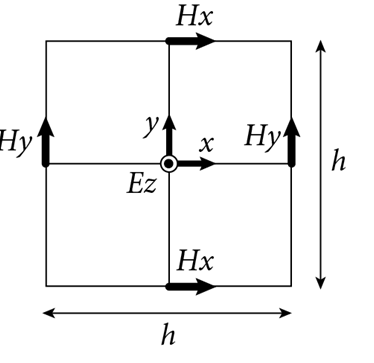
\includegraphics{yee-cell-ez.png}
	\caption{2D $TM_Z$ Yee Cell}
	\label{fig:yeecell}
\end{figure}

More formally, we may expand the $E_Z$ wave equation, arriving at:

\begin{equation} \label{eq:ezupdate}
{E_z}_{i,j}^{t+1} = C_a * {E_z}_{i,j}^{t} 
+ C_b * ({H_x}_{i,j+\frac{1}{2}}^{t+\frac{1}{2}} - {H_x}_{i,j-\frac{1}{2}}^{t+\frac{1}{2}})
+ C_b * ({H_y}_{i+\frac{1}{2},j}^{t+\frac{1}{2}} - {H_xy}_{i-\frac{1}{2},j}^{t+\frac{1}{2}})
\end{equation}

Similarly, the equations for the coupled fields $H_x$ and $H_y$ may be expressed as:
\begin{equation} \label{eq:hxupdate}
{H_x}_{i,j}^{t+1} = D_a * {H_x}_{i,j}^{t} + D_b * (
{E_z}_{i,j+\frac{1}{2}}^{t+\frac{1}{2}} 
-
{E_z}_{i,j-\frac{1}{2}}^{t+\frac{1}{2}}
)  
\end{equation}

\begin{equation} \label{eq:hyupdate}
{H_y}_{i,j}^{t+1} = D_a * {H_y}_{i,j}^{t} + D_b * (
{E_z}_{i+\frac{1}{2},j}^{t+\frac{1}{2}} 
-
{E_z}_{i-\frac{1}{2},j}^{t+\frac{1}{2}}
)  
\end{equation}

\iffalse
From Nathan:

You need to expand this a fair amount more.  You need to at minimum define all of the terms in these equations.  A paragraph or two on how a full domain is discritized, and how a simulation steps in 1/2 detla T steps is important.  

This will be important in the discussion between CPU and GPU architectures as you want to list how with FDTD you calcuate an entire time step, or 'frame' over the entire phyisical domain before moving on to the next frame.  You can state here how the updates of frames are independent of other calculations done during that same frame
\fi

\begin{table}[h!]
	\centering
	\caption{FDTD Equation Terms}
	\label{tab:modelColorComponentUsage}
	\begin{tabular}{l | c | l}
		Symbol	& Definition & Description \\
		\hline				\\										 	 
		$dx$ 	& $\frac{\lambda}{10}$ 			& Spatial step as a function of max source  fundamental frequency 					\\
		$dt$ 	& $\frac{dx}{\sqrt{n}} * 0.9$		& Time step between frame updates, where $n$ is the domain dimensionality \\		$C_a$	& $\frac{1}{\epsilon_0}$ & Permittivity of free space	\\
		$C_b$	& $\frac{dt}{dx}  \frac{1}{\sqrt{\epsilon_0 \epsilon_r}}$ & Permittivity at the location $i,j$\\
		$D_a$	& $\frac{1}{\mu_0}$	& Permeability of free space \\
		$D_b$	& $\frac{dt}{dx}\frac{1}{\sqrt{\mu_0 \mu_r}}$	& Permeability at the location $i,j$\\
		$i$, $j$ 	& &	Field element location within the domain  \\
		$t$   	& &	Current time step ($t_E = t_H \frac{+}{-}\frac{1}{2}$) \\
		$E_Z$ 	& & Electric field amplitude in $Z$ \\
		$H_X$ 	& & Magnetic field amplitude in $X$ \\
		$H_Y$	& & Magnetic field amplitude in $Y$ \\
	\end{tabular}
\end{table}

Since Maxwell's equations are scale-invariant, GoLightly substitutes 1 for constants such as $C$, $\mu_0$ and $\epsilon_0$. The $\frac{0.9}{\sqrt{2}}$ scalar in $dt$ prevents aliasing, and corrects for simulation dimensionality\footnote{This value should be $\frac{0.9}{\sqrt{n}}$, where $n$ is 3 for a 3D domain, 2 for a 2D domain and 1 for a 1D domain.} 

In equations \ref{eq:ezupdate}, \ref{eq:hxupdate} and \ref{eq:hyupdate}, note that each $E_{i,j}^{t+1}$ field update depends only upon the previous $E$ value ($E_{i,j}^{t}$), and the previous adjacent $H$ values ($H_X^{t+\frac{1}{2}}$ and $H_Y^{t+\frac{1}{2}}$). This allows each field component to be updated without regard for any other value in the same field. As such, $E$ field values in any order without the risk of a race condition. The same principle applies to $H$-field updates.  

\section{Leap Frog: Stepping in Space and Time}

In equations \ref{eq:ezupdate}, \ref{eq:hxupdate} and \ref{eq:hyupdate}, note the presence of a "half step" in time ($F^{t + \frac{1}{2}}$) and space $F_{i \frac{+}{-}\frac{1}{2},j \frac{-}{+}\frac{1}{2}}$.

This $t\frac{+}{-}\frac{1}{2}$ represents the temporal step size between an $E$-field update and the next $H$-field update,and visa-versa. Similarly, the spatial offset $x\frac{+}{-}\frac{1}{2}$ represents the distance between an $E$-field component and its adjacent, dependent $H$ values.


\begin{figure}[H]
	\centering
	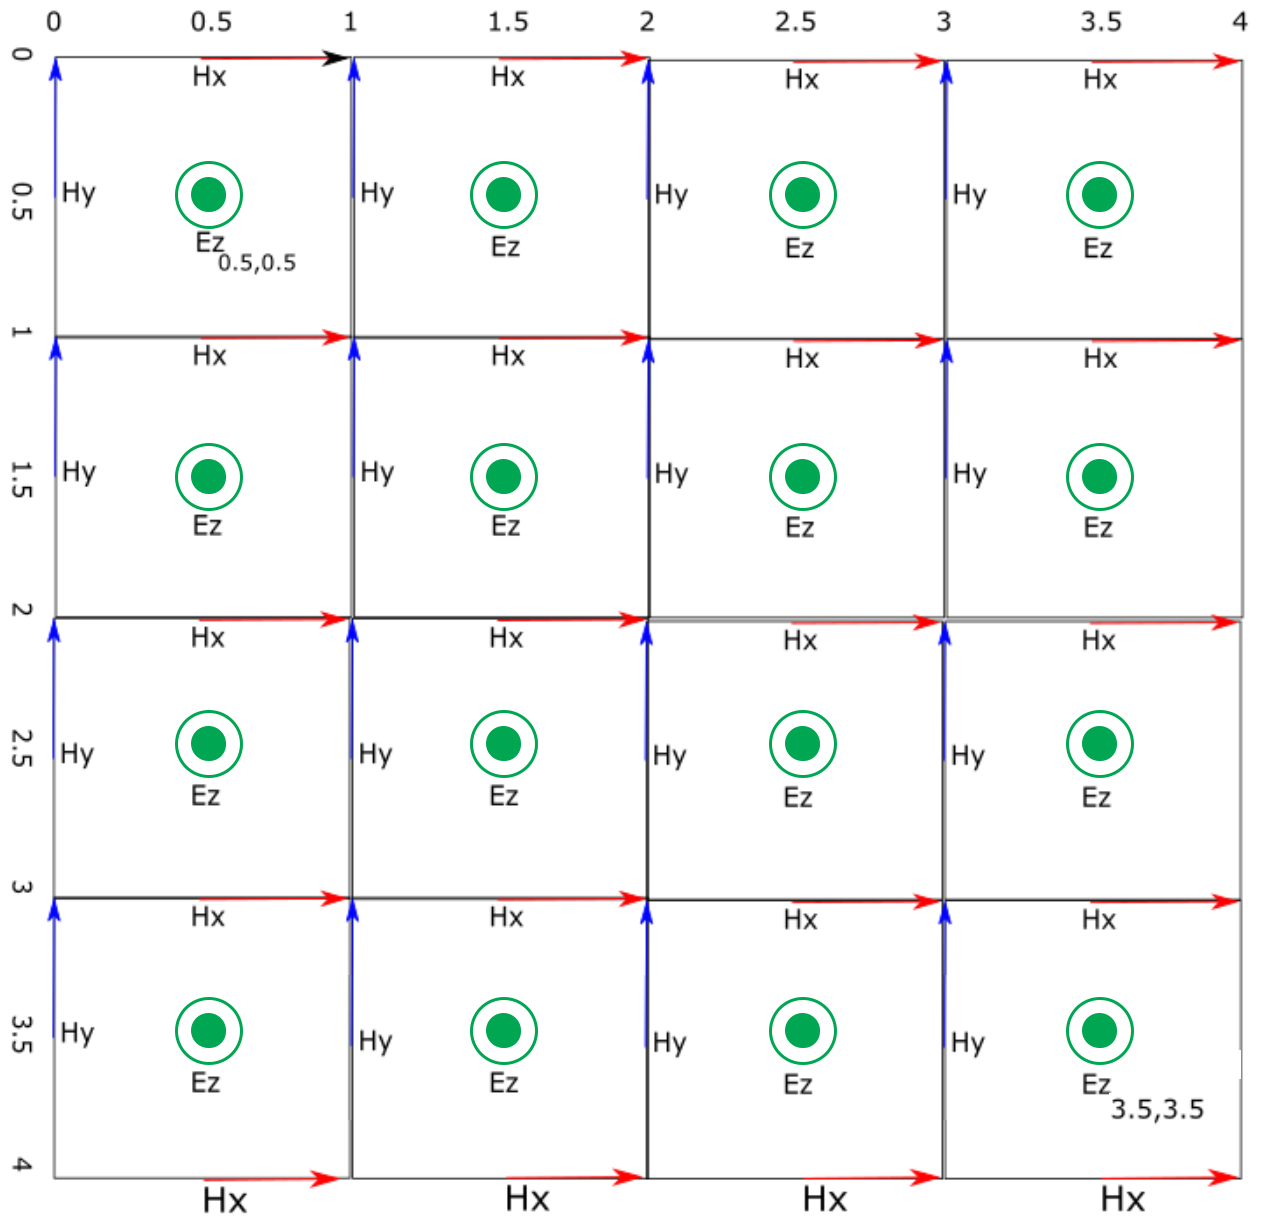
\includegraphics[width=15cm,keepaspectratio]{YeeMesh.png}
	\caption{4x4 Yee Lattice}
	\label{fig:yeeLattice}
\end{figure}

The spatial relationship between $E$ and $H$ grids is illustrated in the Yee lattice in \autoref{fig:yeeLattice}. Note that each $E_Z$ component is in the middle of a cell, at the $(i + \frac{1}{2}, j + \frac{1}{2})$ position where ($i,j$) is  the upper-left corner of the cell. $H$ components, however, are positioned at integer coordinates.

This arrangement reflects the manner in which a wave will propagate through the domain. In the half time step between $E$ and $H$ updates, the wave moves one half-cell. If the $E$ and $H$ components were coincident, the simulation would degrade to a large collection of individual points rather than a discretized domain.


\section{Boundary Conditions}

Recall the $H_Y$ update equation \autoref{eq:hyupdate}, and note that it depends on two adjacent $E_Z$ values on the $X$ axis. The finite grid does not contain enough information to update the $H$ values that lie on the outside of the domain. For instance, ${H_Y}_{0,\frac{1}{2}}$ requires ${E_Z}_{\frac{1}{2},\frac{1}{2}}$ and \bm{${E_Z}_{-\frac{1}{2},\frac{1}{2}}$}.

Since the position $(-\frac{1}{2},\frac{1}{2})$ does not exist, the simulator cannot update this value. The simulator must take this case into account by implementing some sort of absorbing boundary condition, or the wave will reflect from the boundaries. 

We implement the Perfectly Matched Layer (PML) as described in \cite{BERENGER1994185}. 

A detailed explanation of PML is beyond the scope of this thesis. In practice, PML adds imaginary hyperplanes orthogonal to each field in the simulation. In the boundary regions, power couples between $E$ and $H$ as expected, but \emph{also} couples into those hyperplanes. Unlike the $E$ and $H$ interdependence, though, the transfer is one-way. Cells in the PML hyperplanes "contain" materials which force the coupled power to decay over a number of layers. In our implementation, we use 10 PML layers as experimentation showed this to provide the most satisfactory results.



\section{FDTD in SIMD}

FDTD's leap-frog update method, whereby E fields and H fields are successively calculated, is well-suited to a GPU implementation. E field values depend on adjacent H field values, and visa-versa. Since the E-field update equation requires knowledge only of the H field state and previous E field state, each field component can be calculated independently with no opportunity for a pipeline stall or race condition. 

